\section{L'Œdème Pulmonaire d'Immersion (OPI)}

\begin{frame}{Mécanisme de l'OPI}
  \begin{columns}[c]
    \begin{column}{0.55\textwidth}
      \begin{block}{Définition}
        Inondation brutale des alvéoles par du \textbf{plasma sanguin}.
        \small{Ce n'est pas une entrée d'eau, mais une fuite interne.}
      \end{block}
      
      \textbf{Le mécanisme physiologique :}
      \begin{enumerate}
        \item Immersion $\Rightarrow$ \textbf{Blood Shift} (sang chassé vers le thorax).
        \item Augmentation de la pression dans les capillaires pulmonaires.
        \item Rupture de la \textbf{barrière alvéolo-capillaire}.
      \end{enumerate}
    \end{column}
    
    \begin{column}{0.45\textwidth}
      \centering
      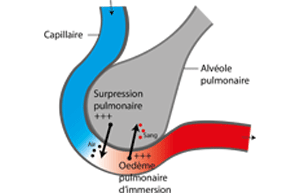
\includegraphics[width=\textwidth]{images/infos-opi}
      \tiny{\textit{Passage du plasma vers l'alvéole (Défaillance barrière)}}
    \end{column}
  \end{columns}
\end{frame}

\begin{frame}{Facteurs favorisants (Le profil à risque)}
  Contrairement à la surpression, l'OPI est souvent lié à la condition du plongeur.
  
  \begin{alertblock}{Facteurs aggravants (Cumulatifs)}
    \begin{itemize}
      \item \textbf{Froid} (Vasoconstriction périphériques).
      \item \textbf{Effort physique} important (palmage soutenu).
      \item \textbf{Hypertension artérielle} (HTA) et problèmes cardiaques.
      \item \textbf{Stress} (Augmentation rythme cardiaque).
    \end{itemize}
  \end{alertblock}

  \begin{block}{Autre facteur identifié}
    \begin{itemize}
      \item Âge (> 40-50 ans).
    \end{itemize}
  \end{block}
\end{frame}

\begin{frame}{Symptômes et Conduite à tenir}
  \begin{columns}[T]
    \begin{column}{0.45\textwidth}
      \textbf{Symptômes :}
      \begin{itemize}
        \item Sensation d'étouffement, dyspnée.
        \item \textbf{Toux} irrésistible pendant la plongée.
        \item Bruits respiratoires (gargouillis).
        \item \textbf{Crachats mousseux et rosés} (Hémoptysie).
      \end{itemize}
      
      \begin{alertblock}{Aggravation}
        Les symptômes \textbf{s'aggravent à la remontée}.
      \end{alertblock}
    \end{column}
    
    \begin{column}{0.45\textwidth}
      \begin{block}{Conduite à tenir}
        \begin{enumerate}
          \item \textbf{Arrêt de tout effort} immédiat.
          \item Remontée assistée calme (éviter la panique).
          \item En surface : Oxygénothérapie (O$_2$).
          \item Appel des secours (CROSS/VHF) $\Rightarrow$ \alert{\textbf{URGENCE VITALE}}.
        \end{enumerate}
      \end{block}
    \end{column}
  \end{columns}
\end{frame}